\section{\tc Design}

In this section, we discuss the general design of \tc. First we present a strawman architecture that illustrates some of the technical challenges that arise in the design of \tc. We then present our \tc architecture, describing the front-end (blockchain) and back-end (off-chain) components, the data flows among them, and the security model underpinning our design.

\subsection{Strawman architecture}

Here we sketch a simple (but, as we show, na\"{i}ve) strawman architecture that provides authenticated data feeds along with accompanying attestations. To harmonize with terminology introduced shortly in the paper, we refer to the untrusted component of a \tc host as the \medname and the code running in an SGX enclave as the \encname.

The strawman solution is as follows:

\begin{itemize}[leftmargin=5mm]
\item
{\bf Monitor and relay.}
The \tc system
monitors the blockchain for 
datagram requests. A contract \reqcont 
requests a datagram by including a distinguished message in its state (e.g., ``\tc service \#123 request:''), along with
a specification \dgform of the requested datagram.
Monitoring happens in the \medname, which controls the network stack. The
\medname forwards ${\sf params}$ 
to the \encname.
\item
{\bf Securely fetch feed.}
Based on the \dgform, the \encname contacts a data source, establishing an HTTPS channel to a suitable target web page $\weburl$ (which might, e.g., be specified in \dgform). 
The \encname verifies that the validity of the certificate for the host serving \weburl.
It then fetches page contents, parses them, and extracts a datagram \dgm as specified in \dgform.

Finally, the \encname produces an attestation $\att$ on: its code in the enclave, $\dgform$, a timestamp $T$ on the fetched data, and $\dgm$. 
It sends $\att$ to $\reqcont$.
\item
{\bf Verify}.
\reqcont verifies the attestation $\att$. If successful, \reqcont consumes \dgm (potentially matching \dgform against an internal queue of datagram requests).
\end{itemize}

This strawman scheme has a few nice features: conceptual simplicity, no need to maintain a \tc contract on the blockchain, and the ability for \reqcont to check the freshness of \att. It has a few serious drawbacks, however.

\paragraph{Problems with the strawman scheme.}
Our strawman scheme is unworkable for several reasons. First, verification of \att in the requesting contract \reqcont is not practical. Although SGX provides a 
trusted clock, the clock does not provide absolute time, but only time relative to a host-specific reference point.
Thus it is not clear in our strawman scheme how to produce a timestamp $T$ in absolute time. Futhermore, in Ethereum, opcodes for in-contract cryptographic operations are very limited and do not support the proprietary EPID group-signature scheme present in SGX attestations. While achievable in principle, as the Ethereum virtual machine is Turing-complete, verification of attestations would impose prohibitively expensive gas costs on \reqcont. 

To address these problems, our \tc architecture supports only off-chain verification of attestations.

Another problem with our strawman scheme is that it lacks an on-blockchain mechanism to enforce payment for datagrams. It is desirable for \tc to accept payments via a smart contract in order to permit payment in the system's cryptocurrency (e.g., Ether) and to ensure a {\em fair exchange} between payments and datagrams. Even a not-for-profit \tc service might accept small gas payments to cover the cost of datagram transmission. Without enforcement of fair exchange, relying contracts or the \tc service would risk being defrauded by the other party. \tc could attempt to deliver datagrams only to contracts whose code guarantees payment to \tc, but verifying this property even in templated code would be challenging, given the many complicated dependencies in a smart-contract system (e.g., a contract might attempt to make payment but lack gas or ether). 

To address these problems, our \tc architecture uses a smart contract \tcont as a blockchain front end.

\subsection{The \tc architecture}

The \tcs system includes three main components: The \tcontract (\tcont), the \encname, and the \medname. The \encname and \medname reside on the \tc server, while the \tcontract  resides on the blockchain. An architectural schematic showing the roles of these components is given in Figure~\ref{fig:overview}.

\vspace{-2mm}
\begin{figure}[h!]
\centering
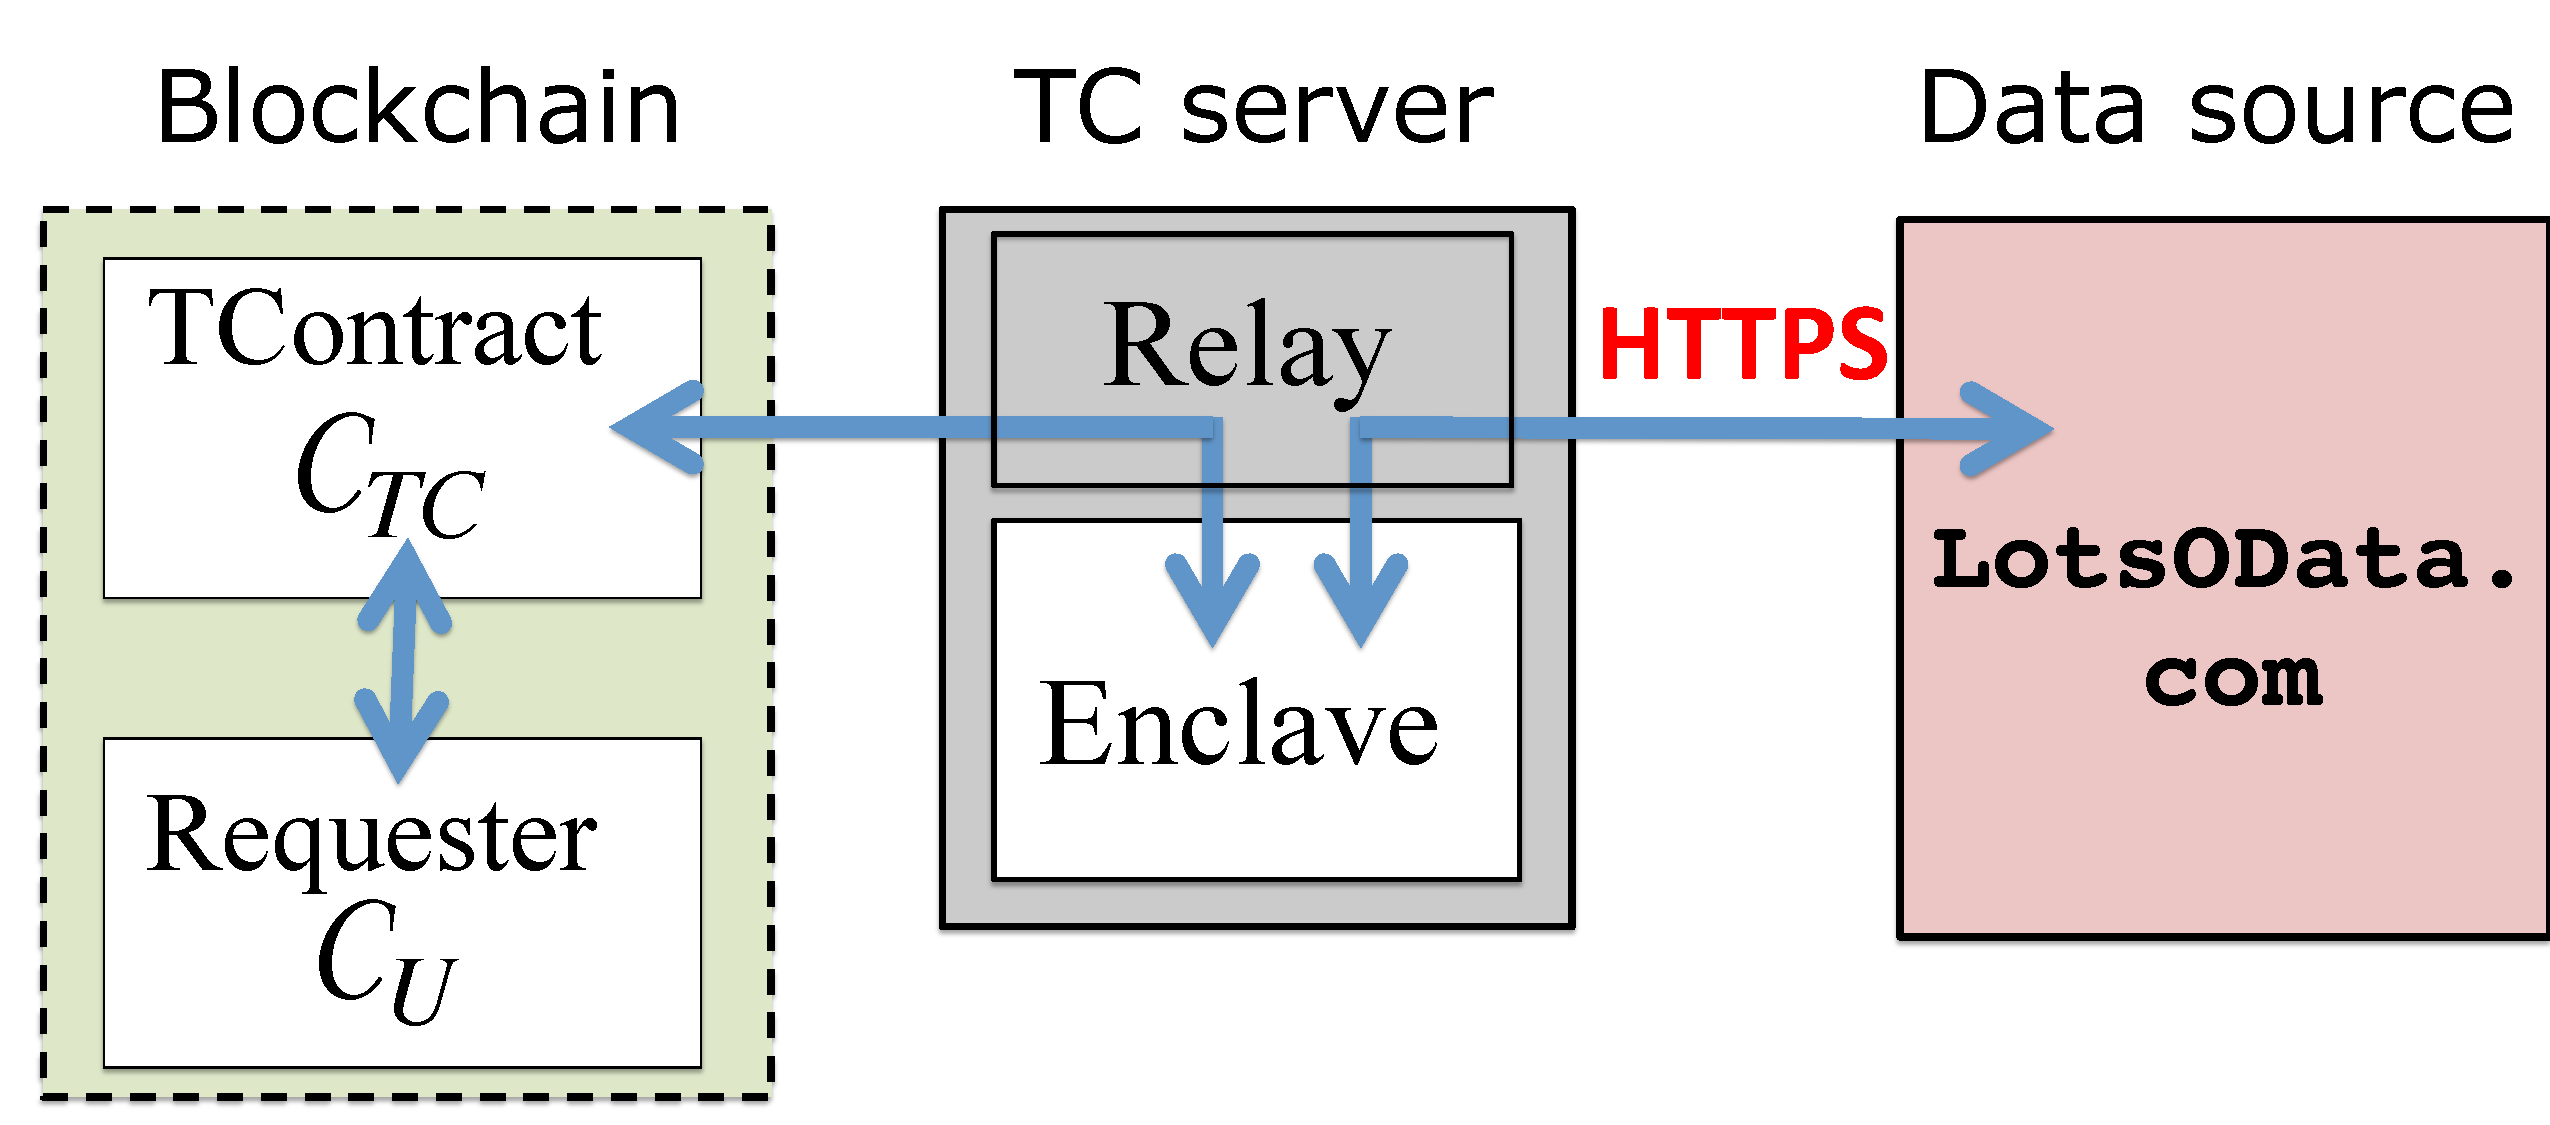
\includegraphics[width=\columnwidth]{figures/OverviewFig}
\caption{{\bf Basic Town Crier architecture.}}
\label{fig:overview}
\end{figure}
\vspace{-2mm}

\paragraph{The \tcontract (\tcont).} The \tcontract (denoted by \tcont) is a smart contract that acts as the blockchain front end of the \tc service. It is designed to present a simple API to a relying contract \reqcont for its requests from \tc. Very simply, \tcont accepts datagram requests from a requester \reqcont and returns corresponding datagrams from \tc. Additionally, \tcont manages \tc monetary resources, which in Ethereum take the form of ether (money) and gas (``fuel'' for contracts).

\paragraph{The \encname.}
The \encname ingests and fulfills datagram requests from the blockchain. To obtain the data for inclusion in datagrams, it queries external data sources, specifically HTTPS-enabled internet services. It returns a datagram to a requesting contract \reqcont as a digitally signed blockchain message. The \encname runs in an SGX enclave, and is thus secured against an adversarial OS as well as other process on the host. 

\paragraph{The \medname.} As an enclave process, the \encname lacks direct network access. Thus the \medname handles bidirectional network traffic on behalf of the \encname. Specifically, the \medname provides network connectivity from the \encname to three different types of entities: 

\begin{enumerate}
\item {\em The Blockchain (the Ethereum system):}  The \medname scrapes the blockchain in order to monitor the state of the \tcontract  \tcont. In this way, it performs implicit message passing from \tcont to the \encname, as neither component itself has network connectivity. Additionally, the \medname places messages emitted from the \encname (datagrams) on the blockchain.
\item {\em Clients:} The \medname runs a web server to handle off-chain service requests from clients, specifically, requests for attestations from the \encname. As we soon explain, an attestation provides a unique public key for the \encname instance to the  client and proves that the \encname is executing correct code in an enclave and that its clock is correct in terms of absolute (wall-clock time). A client that successfully verifies an attestation can then safely create a relying contract \reqcont that uses the \tc.
\item {\em Data sources:} The \medname relays traffic to and from data sources (HTTPS-enabled servers) queried by \encname. 
\end{enumerate}

The \medname is an ordinary user-space application. It does not benefit from integrity protection by trusted hardware and thus, unlike the \encname, can be subverted by an adversarial OS on the \tc server, causing network delays or failures. As we explain in detail later in the paper, however, a key design aim of \tc is that \medname should be unable to cause incorrect datagrams to be produced or users to lose fees paid to \tc for datagrams (although they may lose gas used to fuel their requests). In general, the \medname~{\em can only mount denial-of-service attacks against \tc}. 

\paragraph{End-to-end datagram processing.}

The lifecycle of a datagram may be summarized in the following steps:

\begin{itemize}
\item {\bf Initiate request.} \reqcont sends a datagram request to \tcont on the blockchain.

\item {\bf Monitor and relay.} The \medname monitors \tcont and relays incoming datagram requests to the \encname.

\item {\bf Securely fetch feed.} Based on \dgform, the \encname contacts a data source via HTTPS and obtains the requested datagram. It forwards the datagram via the Relay to \tcont.

\item {\bf Return datagram.} \tcont checks the correctness of \dgform and returns the datagram to \reqcont.
\end{itemize}


%In addition to servicing datagram requests, the \encname may be queried by a client to provide an off-chain, hardware-backed attestation $\att$ on the state of the \encname---both its executing code and its clock. It is to support this service that \medname includes a web server. We do not depict this service in Figure~\ref{fig:overview}, and defer its discussion to later in the paper.

We now make this data flow more precise. 

\subsection{Datagram processing: Data flow}

We denote a datagram instance, namely the set of message values associated with a datagram request, by $\dgi$, where $i$ is a unique instance index. (We explain in Section~\ref{sec:implementation} how this index is computed.) 

A datagram request by \reqcont takes the form of a message $\dgi.\dgreq$ to \tcont on the blockchain. This message $\dgi.\dgreq = (\dgi.\dgform, \dgi.\dgpay)$ includes both a specification $\dgi.\dgform$ of the requested datagram (e.g., a stock ticker and desired time) and a payment $\dgi.\dgpay$, which in Ethereum may include gas to cover the execution cost of the request as well as a service fee. \tcont receives a return message $\dgi.\dgret = (\dgi.\dgform, \dgi.\dgm)$ from the $\tc$ service where $\dgm$ contains the data (e.g., the desired stock ticker price). \tcont checks the consistency of $\dgi.\dgform$ on the incoming and outgoing messages, and if they match forwards $\dgi.\dgm$ to \reqcont. Where clear from context, we omit the prefix $\dgi$ from our notation.

Figure~\ref{fig:dataflow} shows the data flows involved in processing a datagram request. For simplicity, the figure omits the \medname, which is only responsible for data passing.


\begin{figure}[h!]
\centering
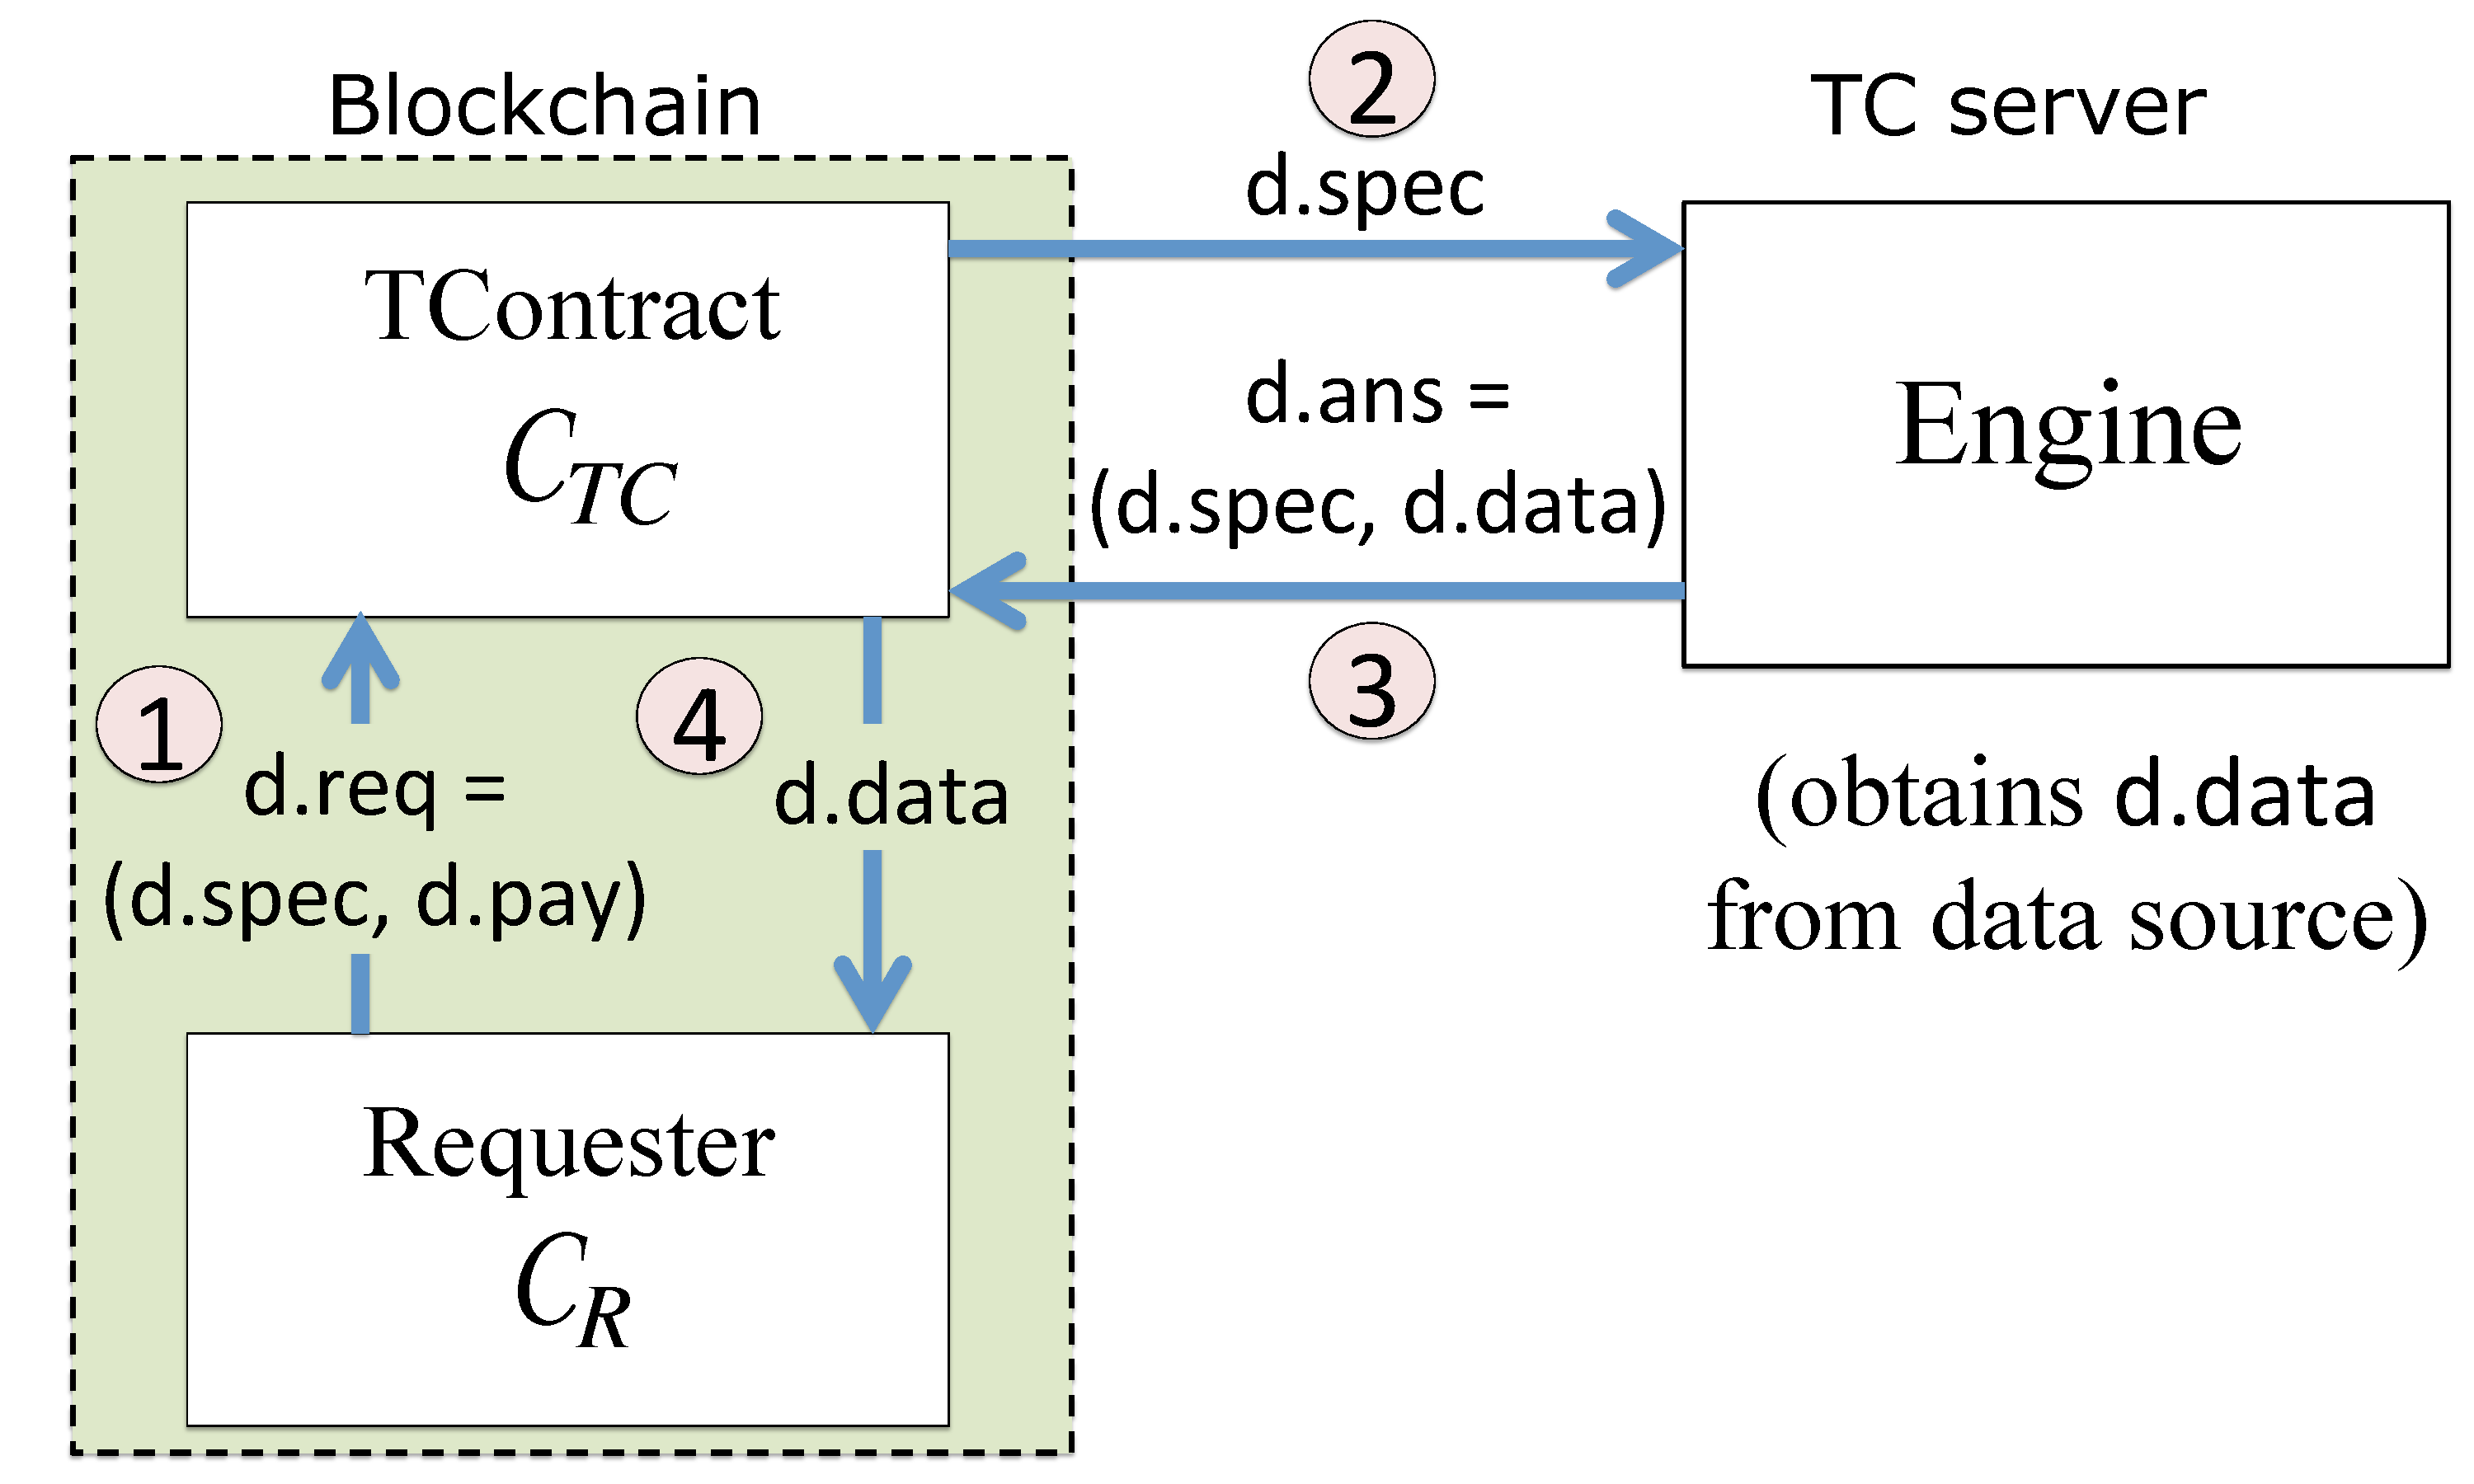
\includegraphics[width=\columnwidth]{figures/DataflowFig}
\caption{{\bf Data flows in datagram processing.}}
\label{fig:dataflow}
\end{figure}


Digital signatures are needed to authenticated messages, such as $\dgret$, entering the blockchain from an external source. We let $(\skTC, \pkTC)$ denote the private / public keypair associated with the \encname for such message authentication. For simplicity, we assume for the time that the \encname can send signed messages directly to \tcont. Later we explain how Ethereum requires a slightly different approach in which \tc sends messages via an Ethereum wallet.

\subsection{Security model}

Here we give an overview of our security model for \tc, providing more details in our security analysis in section~\ref{}. We assume the following:

\begin{itemize}
\item {\em \encname security:} We make three assumptions about \encname : (1) \encname behaves honestly, i.e., correctly executes the \tc protocol; (2) The private key $\skTC$ is known only the \encname; and (3) The \encname has an accurate (internal) real-time clock. (Specifically, the clock is accurate to within XXX, as we show experimentally.)

These three properties are achieved under the security model presumed by SGX. Specifically, they are asserted by an SGX attestation $\att$ generated on an instance of the \encname. We make the additional simplifying assumption that an attestation remains valid throughout its lifetime of use. (Later in the paper, we discuss ways in which later incarnations of Ethereum may support fresher attestations and also issues such as SGX host revocation.)

\item {\em Network communication:} The \medname (and other untrusted components of the \tc server) can tamper with or delay communications to and from the \encname, but cannot otherwise observe or alter the behavior of the \encname. This assumption is again consistent with the SGX security model. Thus the \medname is subsumed by an adversary that controls the network. 

\item {\em Blockchain communication:} Message sources are authenticable, i.e., the originating blockchain address of a message can be correctly identified, and messages are integrity protected, but not confidential. This assumption includes messages sent from the \encname, whose public key $\pkTC$ is bound in \tc to a blockchain account. 
\end{itemize}












